\section{Introducción y Criterios de Selección}
Para la construcción de un equipo o instalación en la industria química se ha de elegir un material capaz de soportar las condiciones exigentes en las que prestará su servicio (presión, temperatura, fluidos agresivos, esfuerzos mecánicos y vibraciones).

En términos generales, los \textbf{materiales más resistentes a la corrosión y al ataque de agentes químicos presentan una baja resistencia mecánica} o un coste económico excesivamente elevado. Si la elección se realiza atendiendo exclusivamente a la resistencia química, las soluciones suelen resultar inviables económicamente. Por ello, se debe alcanzar una \textbf{solución de compromiso} de modo que el coste global del equipo sea asumible a lo largo de su vida útil.

En muchos casos de diseño en Ingeniería Química, la elección se realiza seleccionando un material de elevada resistencia mecánica y coste moderado (como los aceros al carbono), compensando las pérdidas previsibles por ataque químico mediante un \textbf{espesor de sobreespesor por corrosión} (\textit{corrosion allowance}).

Un \textbf{material ideal para la construcción de una planta química} debe satisfacer los siguientes requisitos:
\begin{itemize}
    \item \textbf{Inercia química:} No ser atacable por el sistema químico que contiene ni degradar el medio circundante.
    \item \textbf{Pureza de proceso:} No catalizar reacciones indeseadas ni contaminar el producto de reacción.
    \item \textbf{Resistencia mecánica adecuada:} Soportar tensiones estáticas, cíclicas o de impacto a las temperaturas de operación.
    \item \textbf{Viabilidad económica y tecnológica:} Coste de adquisición asumible y facilidad para ser conformado, soldado y mecanizado.
\end{itemize}
\nt{Es decir, los materiales deben ser resistentes a la corrosión y a su vez que tengan una resistencia mecanica elevada, debido a que es realmente inusual que cumpla ambas lo que se hace es llegar a un compromiso basandonos en la economia y en la viabilidad tecnologica que cumplan ambos criterios, se seleccionara el espesor calculado del material y ademas se le añadira un espesor por corrosión calculado para los años de vida util es decir que el espesor final seleccionado sera la suma de ambos}
\section{Propiedades Mecánicas de los Materiales}

Dentro del conjunto de propiedades de los materiales (mecánicas, térmicas, eléctricas, químicas, etc.), son las \textbf{propiedades mecánicas de resistencia, mecánicas superficiales, tecnológicas y la resistencia química} los factores determinantes en el diseño mecánico de equipos e instalaciones de proceso.

El \textbf{comportamiento mecánico} refleja la relación funcional entre la fuerza aplicada sobre el componente y la respuesta resistente y deformable que experimenta dicho material. Para evaluar de manera cuantitativa y reproducible este comportamiento se recurre a \textbf{ensayos normalizados}, lo que permite comparar de forma objetiva distintos materiales y calidades comerciales.

\subsection{Factores influyentes en el comportamiento bajo carga}
A la hora de llevar a cabo los ensayos mecánicos y evaluar el servicio de los materiales se deben considerar cuatro factores fundamentales:
\begin{enumerate}
    \item \textbf{Naturaleza de la carga aplicada:}
          \begin{itemize}
              \item \textit{Tracción:} Fuerzas colineales que tienden a estirar el elemento longitudinalmente.
              \item \textit{Compresión:} Fuerzas que tienden a acortar el elemento en la dirección de aplicación.
              \item \textit{Pandeo:} Inestabilidad elástica por compresión en elementos esbeltos (Se da cuando la relación longitud respecto sección es elevada).
              \item \textit{Flexión:} Momentos flectores que generan tracción en una cara y compresión en la opuesta.
              \item \textit{Torsión:} Momentos torsores que provocan tensiones cortantes alrededor del eje longitudinal.
              \item \textit{Corte o cizalladura:} Fuerzas paralelas y coplanares a la sección resistente que tienden a deslizar planos adyacentes.
          \end{itemize}

          \begin{figure}[H]
              \centering
              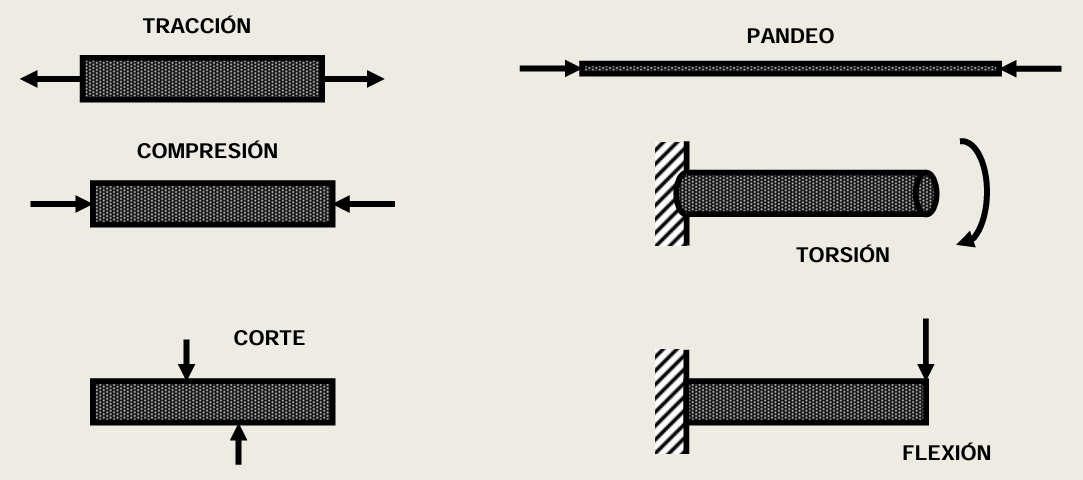
\includegraphics[width=0.7\textwidth]{Tipos_carga.png}
              \caption{Fuente: Transparencias Asignatura}
              \label{fig:tipos_carga}
          \end{figure}

    \item \textbf{Superficie y distribución de aplicación:} Carga concentrada (puntual), uniformemente distribuida o uniformemente variada.
          \begin{figure}[H]
              \centering
              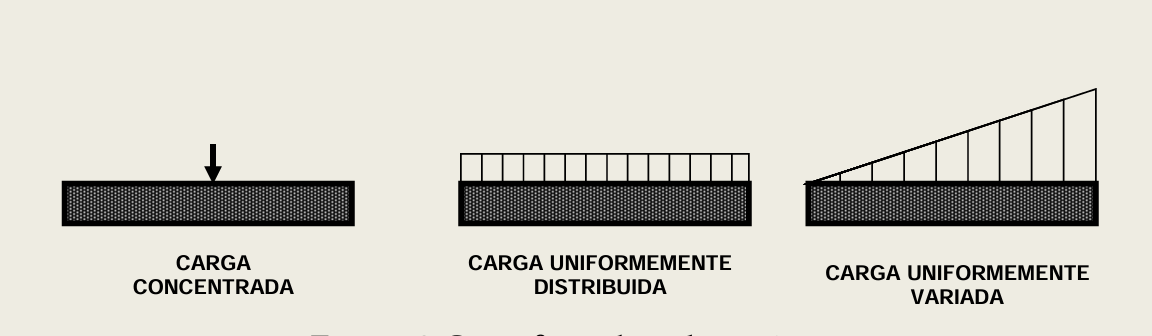
\includegraphics[width=0.7\textwidth]{superficie_aplicacion.png}
              \caption{Fuente: Transparencias Asignatura}
              \label{fig:superficie_aplicacion}
          \end{figure}
    \item \textbf{Tiempo y régimen de duración:}
          \begin{itemize}
              \item \textit{Carga constante o estática:} Aplicada de forma suave y mantenida en el tiempo.
              \item \textit{Carga progresiva:} Crecimiento lento y continuo de la solicitación.
              \item \textit{Carga repetitiva o cíclica:} Cargas variables en el tiempo que oscilan o fluctúan (origen de la fatiga).
              \item \textit{Carga alternativa:} Fluctuación completa del sentido de la carga (de $+P$ a $-P$).
              \item \textit{Carga de choque o impacto:} Aplicación brusca en fracciones de segundo con elevada transferencia de energía cinética.
          \end{itemize}
    \item \textbf{Condiciones del medio:} Temperatura de servicio (criogénica o elevada), exposición a atmósferas húmedas, salinas o fluidos corrosivos bajo tensión.
\end{enumerate}
\subsection{propiedades mecánicas}
El comportamiento mecánico de un material refleja la relación entre la fuerza aplicada y la respuesta del material a su deformación (resistencia que ofrece a la aplicación de la carga).
Las propiedades mecánicas de los materiales se determinan realizando ensayos normalizados que permiten comparar entre si el comportamiento de distintos materiales.
\begin{itemize}
    \item \textbf{Propiedades mecánicas de resistencia:} Comportamiento frente a esfuerzos axiales, cortantes o flectores (tracción, compresión, fatiga, termofluencia).
    \item \textbf{Propiedades mecánicas superficiales:} Resistencia a la deformación plástica localizada, penetración y rayado (dureza y resistencia al desgaste abrasivo).
    \item \textbf{Propiedades tecnológicas:} Capacidad del material para someterse a procesos de conformado y transformación (soldabilidad, flexión, embutición, abocardado).
\end{itemize}
Algunas normativas que lo regulan son ASME, ASTM y ISO.
\subsection{Conceptos Básicos de Elasticidad y Deformación}

\subsubsection{Tensión o Esfuerzo ($\sigma$)}
\dfn{Tensión o esfuerzo nominal}{Es la resistencia interna que ofrece una sección del material perpendicular a la carga aplicada. La tensión o esfuerzo que sufre un elemento ($\sigma$) es igual al cociente entre la fuerza uniaxial media y la sección transversal original de la barra.}

Considerando una barra o probeta prismática/cilíndrica de longitud inicial $l_0$ y sección transversal inicial $A_0$ sometida a una fuerza uniaxial normal $P$, la tensión $\sigma$ viene dada por:
\begin{equation}
    \sigma = \frac{P}{A_0}
    \label{eq:tension_nominal}
\end{equation}
\nt{La tensión ingenieriel siempre esta referida a la sección inicial}
\textbf{Unidades de tensión y esfuerzo habituales en ingeniería:}
\begin{itemize}
    \item \textbf{Sistema Internacional (SI):} Pascal ($\text{Pa} = \text{N}/\text{m}^2$). En ingeniería mecánica se emplean los múltiplos:
          \begin{equation*}
              1\text{ MPa} = 10^6\text{ Pa} = 1\text{ N}/\text{mm}^2, \qquad 1\text{ GPa} = 10^9\text{ Pa} = 10^3\text{ N}/\text{mm}^2
          \end{equation*}
    \item \textbf{Sistema Técnico:} Kilogramo-fuerza por centímetro cuadrado ($\text{kgf}/\text{cm}^2$) o por milímetro cuadrado ($\text{kgf}/\text{mm}^2$), donde $1\text{ kgf} \approx 9.80665\text{ N}$.
    \item \textbf{Sistema Anglosajón (U.S. Customary Units):} Libra-fuerza por pulgada cuadrada ($\text{psi} = \text{lbf}/\text{in}^2$) o miles de psi ($\text{ksi} = 10^3\text{ psi}$):
          \begin{equation*}
              1\text{ psi} \approx 6.89476 \times 10^3\text{ Pa}, \qquad 1\text{ ksi} \approx 6.89476\text{ MPa}
          \end{equation*}
\end{itemize}

\subsubsection{Deformación y Deformación Unitaria ($\varepsilon$)}
\dfn{Deformación}{Al aplicar una carga uniaxial $P$, el elemento experimenta una variación dimensional en la dirección longitudinal de la fuerza denominada alargamiento o deformación total $\delta = l - l_0$. Es decir es el incremento de la longitud de la barra o probeta inicial. }

\dfn{Deformación Unitaria}{En ingeniería se define la \textbf{deformación unitaria nominal} ($\varepsilon$) como el cociente entre el incremento de longitud y la longitud inicial de referencia:}
\begin{equation}
    \varepsilon = \frac{\delta}{l_0} = \frac{l - l_0}{l_0} \quad [\text{adimensional, habitualmente expresada en } \% \text{ o en } \text{mm}/\text{mm}]
    \label{eq:deformacion_unitaria}
\end{equation}

\subsubsection{Coeficiente de Poisson ($\nu$ o $\eta$)}
Una deformación longitudinal uniaxial viene invariablemente acompañada por una deformación transversal de sentido opuesto (contracción lateral en tracción, dilatación lateral en compresión). En materiales elásticos homogéneos e isótropos, las deformaciones unitarias transversales en los ejes perpendiculares son iguales ($\varepsilon_x = \varepsilon_y$).

El \textbf{coeficiente de Poisson} se define como el valor negativo del cociente entre la deformación unitaria lateral y la deformación unitaria longitudinal axial ($\varepsilon_z$):
\begin{equation}
    \nu = -\frac{\varepsilon_x}{\varepsilon_z} = -\frac{\varepsilon_y}{\varepsilon_z}
    \label{eq:poisson_ratio}
\end{equation}

Para un material idealmente incompresible bajo deformación elástica (sin variación de volumen), $\nu = 0.50$. En los materiales estructurales y metales de interés en ingeniería mecánica, $\nu$ oscila habitualmente entre $0.25$ y $0.40$ (Tabla~\ref{tab:poisson_valores}).

\begin{table}[H]
    \centering
    \begin{tabular}{lc lc}
        \toprule
        \textbf{Metal / Aleación} & \textbf{Coeficiente $\nu$} & \textbf{Metal / Aleación}     & \textbf{Coeficiente $\nu$} \\
        \midrule
        Aluminio                  & 0.33                       & Latón                         & 0.35                       \\
        Cobre                     & 0.35                       & Magnesio                      & 0.29                       \\
        Níquel                    & 0.31                       & Acero ordinario / estructural & 0.27 -- 0.30               \\
        Titanio                   & 0.36                       & Tungsteno (Wolframio)         & 0.28                       \\
        \bottomrule
    \end{tabular}
    \caption{Coeficientes de Poisson característicos para metales y aleaciones habituales.}
    \label{tab:poisson_valores}
\end{table}

\subsubsection{Deformación Elástica frente a Deformación Plástica}
Al someter a una fuerza de tensión uniaxial $\sigma$, el material sufre deformación, dependiendo de como quede el material despues de retirarla podemos hablar de:

\begin{itemize}
    \item \textbf{Deformación elástica:} Si al retirar la carga el material recupera instantáneamente sus dimensiones iniciales $l_0$.
    \item \textbf{Deformación plástica:} Si al retirar la carga el material experimenta una deformación permanente y residual. Durante esta deformación se ha producido una reorganización estructural del material y los atomos se han desplazado de sus posiciones de equilibrio.
\end{itemize}
\newpage
\section{Ensayo de Tracción}

El ensayo de tracción uniaxial es el procedimiento estándar más importante para determinar cuantitativamente las propiedades mecánicas de resistencia y deformabilidad de los materiales.

Se someten a un lento estiramiento mediante una equipo de ensayo \ref{fig:ensayo_traccion_esquema}, observándose la carga resultante y la deformación unitaria obtenida hasta el momento de la rotura final de la pieza. Debido a que las tensiones son monoaxiales y no poliaxiales tal y como se dan en la realidad
este ensayo \textbf{No proporciona conclusiones definitivas, Pero es clave para comparar diferentes materiales entre si, ademas las condiciones a las que se realiza el ensayo deben estar normalizadas} es decir se usan probetas de dimensiones establecidas, ademas de a una velocidad y temperatura prefijadas.

\begin{figure}[H]
    \centering
    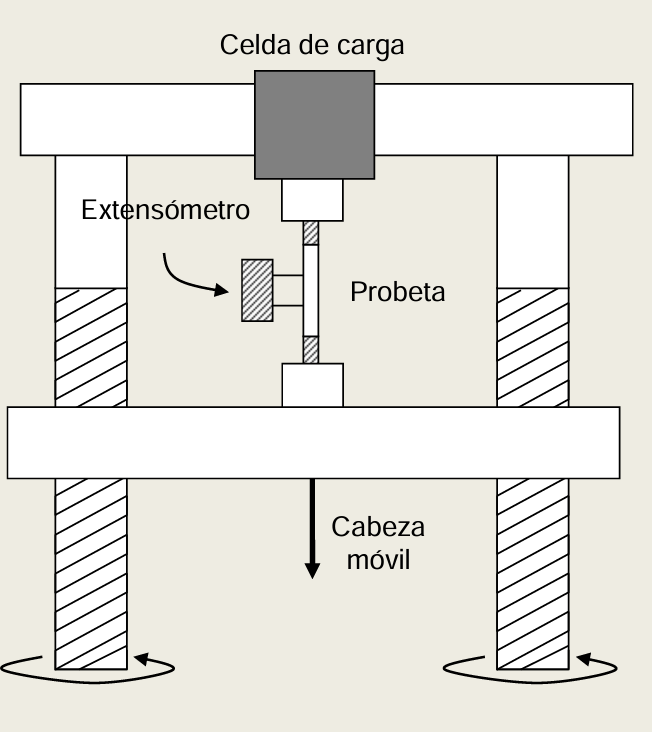
\includegraphics[width=0.7\textwidth]{ensayo_traccion.png}
    \caption{Esquema del ensayo de tracción.\\ Fuente: Transparencias Asignatura}
    \label{fig:ensayo_traccion_esquema}
\end{figure}

\subsection{Probetas Normalizadas (Norma ASTM)}
Para garantizar la reproducibilidad y comparación interlaboratorio, el ensayo se realiza bajo condiciones normalizadas (velocidad de deformación controlada y temperatura ambiente controlada). La Sociedad Americana de Ensayos de Materiales (\textbf{ASTM}) especifica geometrías estandarizadas:
\begin{itemize}
    \item \textbf{Probetas de sección circular:} Utilizadas comúnmente en piezas forjadas, barras y fundiciones. Presentan una longitud calibrada central reducida de diámetro $d_0 = 0.500'' \pm 0.010''$ ($12.7\text{ mm}$) y una longitud de calibración $L_0 = 2.000'' \pm 0.005''$ ($50.8\text{ mm}$). \textcolor{red}{En general, se exige la condición geométrica:} \nt{En caso de que la relación sea mayor}
          \begin{equation}
              \frac{L_0}{d_0} \leqslant 4
          \end{equation}
    \item \textbf{Probetas de sección rectangular:} Utilizadas para ensayos de chapas, perfiles y láminas laminadas, adaptando el espesor al del producto comercial y con transiciones curvas amplias hacia los cabezales de amarre.
\end{itemize}
Los extremos ensanchados de la probeta se sujetan mediante mordazas de cuña, asegurando que la rotura ocurra siempre en la zona central calibrada y no en las proximidades de las mordazas donde se generan concentraciones locales de tensiones.

\subsection{Curva Tensión-Deformación y Puntos Característicos}

Si se coloca la probeta en la máquina de ensayo de tracción y compresión y se aplica gradualmente \textbf{fuerzas de tracción} en los extremos, se puede medir \textbf{el alargamiento total en la longitud patrón para cualquier incremento predeterminado de la carga axial.} Las máquinas llevan generalmente un dispositivo que representa en un diagrama \textbf{la relación entre la carga (P) y el alargamiento ($\delta$).} Normalmente en los diagramas tensióndeformación se representa el \textbf{esfuerzo desarrollado en la probeta ($\sigma$) frente a la deformación unitaria ($\epsilon$)}

\begin{figure}[H]
    \centering
    \includegraphics[width=0.7\textwidth]{diagrama_tension_deformacion.png}
    \caption{Diagrama tensión-deformación para distintos materiales. Fuente: Transparencias Asignatura}
    \label{fig:diagrama_tension_deformacion}
\end{figure}
\begin{itemize}
    \item \textbf{Materiales dúctiles (a)} (ej. aceros de bajo carbono, cobre, aluminio recocido): Presentan un alargamiento elástico inicial lineal, una clara zona de deformación plástica uniforme generalizada, estricción localizada y un elevado alargamiento total antes de la fractura (Punto de rotura).
    \item \textbf{Materiales frágiles (b)} (ej. fundiciones grises, cerámicos, aceros de altísima dureza): Prácticamente no exhiben deformación plástica; la rotura se produce de manera repentina poco después de superado el régimen elástico lineal, con deformación a rotura insignificante.
    \item \textbf{Materiales elastoméricos / polímeros termoplásticos (c):} Muestran curvas no lineales con grandes deformaciones como se aprecia en la gráfica.
\end{itemize}
\nt{En el eje y siempre debe ir la tensión ingenieril es decir respecto a la sección inicial}
Del diagrama se pueden obtener una serie de puntos claves que caracterizan a los materiales como son:
\begin{multicols}{2}
    \begin{itemize}
        \item Límite de proporcionalidad elástico
        \item Límite elástico
        \item Puntos de fluencia
        \item Resistencia máxima a la tracción
        \item Punto de rotura
        \item Ductilidad
        \item Resiliencia
        \item Tenacidad
    \end{itemize}
\end{multicols}
\begin{figure}
    \centering
    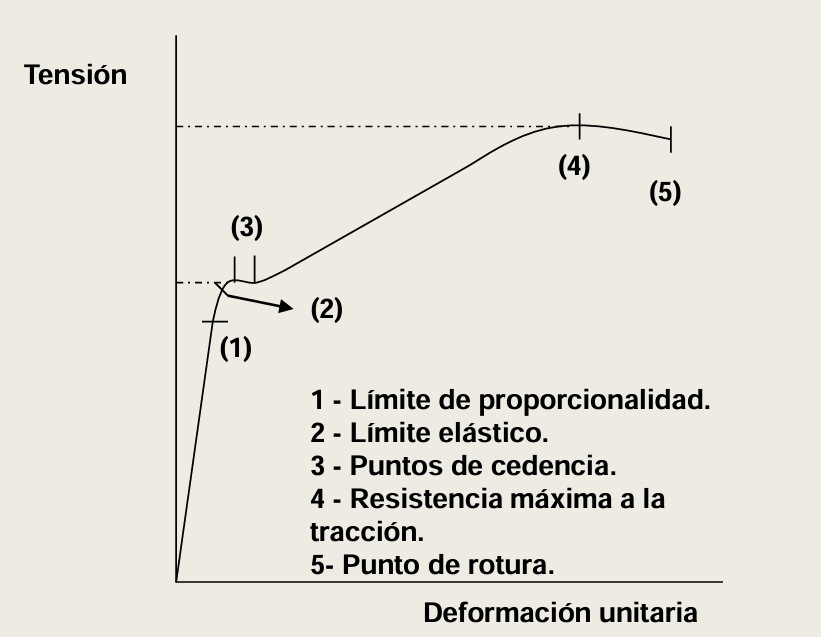
\includegraphics[width=0.7\textwidth]{puntos_diagrama_tension_deformacion.png}
    \caption{Puntos característicos de la curva tensión-deformación del acero.\\ Fuente: Transparencias Asignatura}
    \label{fig:puntos_diagrama_tension_deformacion}
\end{figure}
Estos puntos son importantes, ya que nos permiten determinar la tensión maxima para el diseño del equipo, aunque dependiendo del caso se optará por unos puntos u otros.
\subsubsection{Módulo de Young ($E$) y Límite de Proporcionalidad ($\sigma_{LP}$)}
Es la relacion entre la tensión $\sigma$ y la deformación $\varepsilon$, se calcula en el tramo inicial de la curva donde la relación es estrictamente proporcional cumpliéndose la \textbf{Ley de Hooke}:
\begin{equation}
    \sigma = E \, \varepsilon \quad \Longleftrightarrow \quad \frac{P}{A_0} = E \, \frac{\delta}{L_0}
    \label{eq:hooke_law}
\end{equation}
La constante de proporcionalidad $E$ se denomina \textbf{Módulo de Elasticidad o Módulo de Young}. Representa la rigidez del material frente a la deformación elástica:
\begin{itemize}
    \item Un valor elevado de $E$ indica un material rígido (requiere elevados esfuerzos para sufrir deformación elástica).
    \item Un valor bajo de $E$ describe un material flexible o elástico.
\end{itemize}

\begin{table}[H]
    \centering
    \begin{tabular}{lccc}
        \toprule
        \textbf{Material}                  & \textbf{$E$ ($\text{psi}$)} & \textbf{$E$ ($\text{GPa}$)} & \textbf{$E$ ($\text{Pa}$)} \\
        \midrule
        Cobre recocido                     & $16 \times 10^6$            & $110$                       & $1.1 \times 10^{11}$       \\
        Acero ordinario y de baja aleación & $29 \times 10^6$            & $200$                       & $2.0 \times 10^{11}$       \\
        Aleaciones de aluminio estructural & $10 \times 10^6$            & $70$                        & $0.7 \times 10^{11}$       \\
        Titanio comercial puro             & $15 \times 10^6$            & $105$                       & $1.05 \times 10^{11}$      \\
        \bottomrule
    \end{tabular}
    \caption{Módulos de Young característicos para distintos metales de uso en ingeniería.}
    \label{tab:modulos_young}
\end{table}

\dfn{Límite de proporcionalidad ($\sigma_{LP}$)}{El \textbf{límite de proporcionalidad} ($\sigma_{LP}$) representa el nivel máximo de tensión a partir del cual la relación lineal deja de cumplirse:}
\begin{equation}
    \sigma_{LP} = \frac{P_{LP}}{A_0}
\end{equation}
\imp{La tensión en el límite de proporcionalidad ($\sigma_{LP}$) es la correspondiente al punto donde deja de existir una relación lineal entre el esfuerzo aplicado y la deformación unitaria. $P_{LP}$ es la carga aplicada en el límite de proporcionalidad.}
\textbf{Método de Johnson para determinar $\sigma_{LP}$:} Dado que la desviación de la linealidad puede ser gradual y difícil de discernir visualmente, se emplea el método gráfico de Johnson: se traza una recta $OE$ tangente a la curva en el origen con pendiente $E$, y se define otra recta $OD$ con una pendiente un $50\%$ inferior respecto al eje de esfuerzos (es decir, en una paralela horizontal a distancia $FD = 1.5 \, FE$). Trazando una paralela a $OD$ que sea tangente a la curva de tracción, el punto de tangencia define con rigor el límite de proporcionalidad.
\begin{figure}[H]
    \centering
    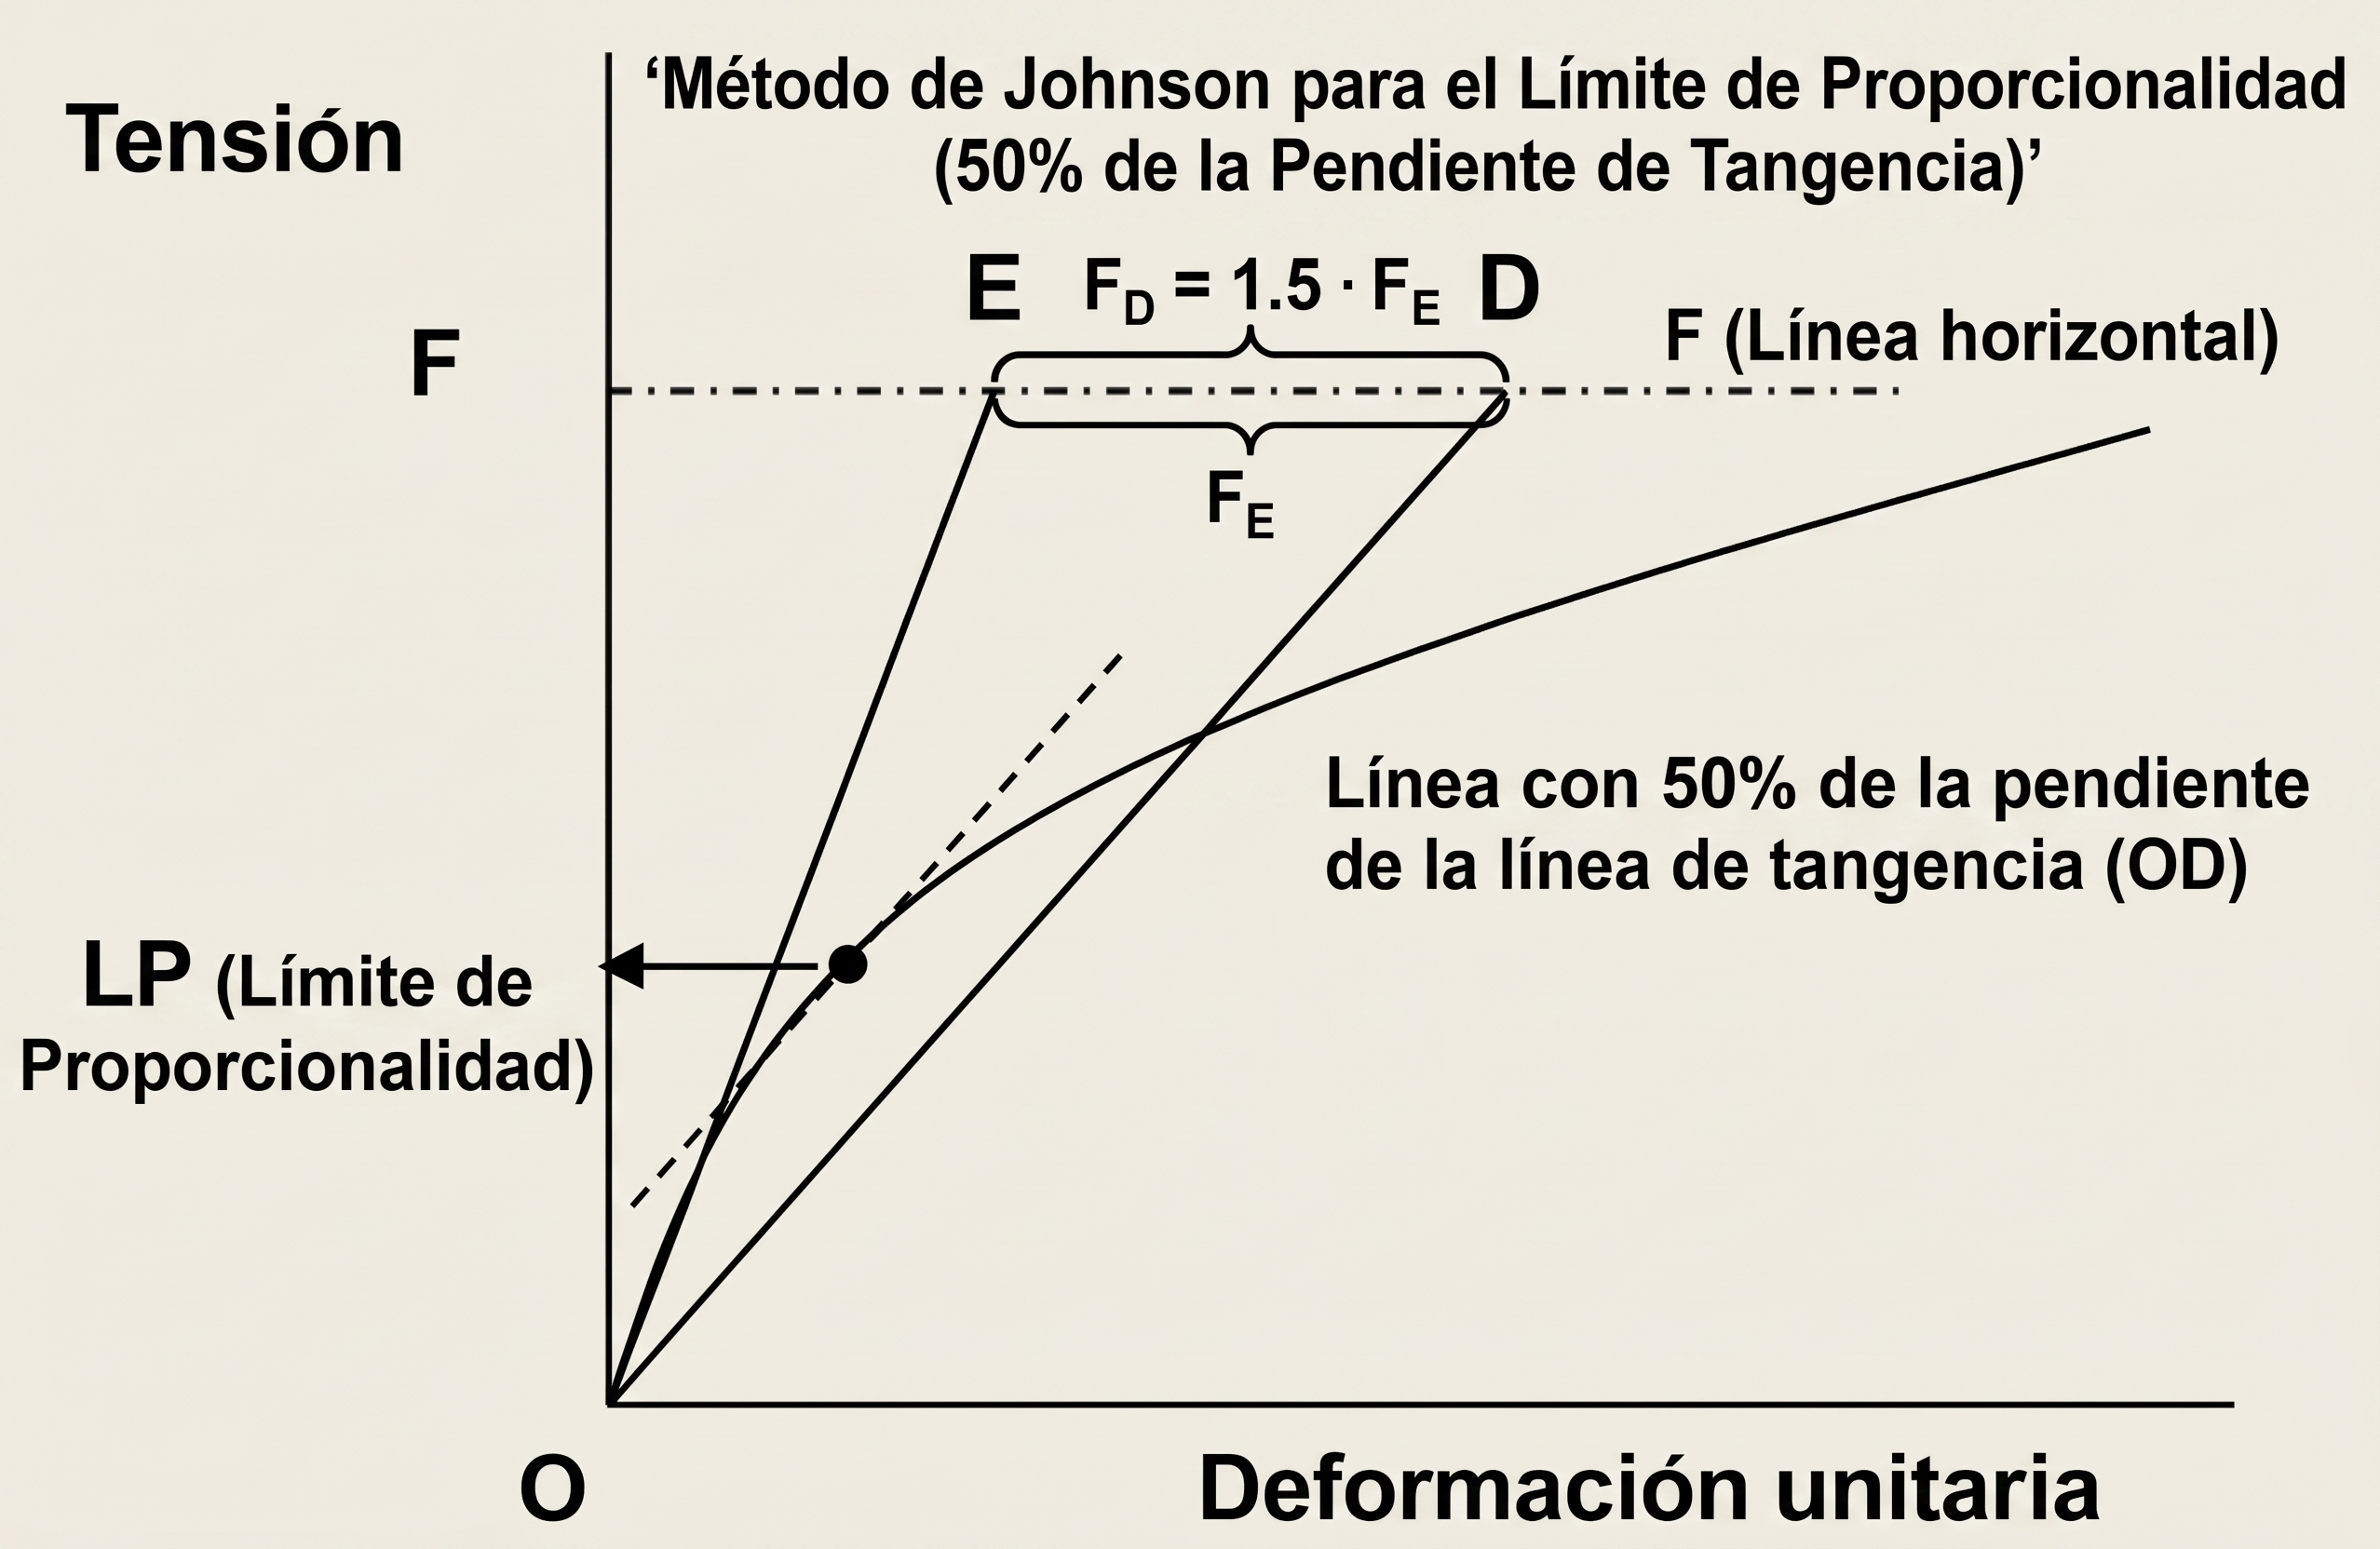
\includegraphics[width=0.7\textwidth]{Gemini_Generated_Image_a8mnpsa8mnpsa8mn.jpg}
    \caption{Método de Johnson para determinar $\sigma_{LP}$. Fuente: Transparencias Asignatura}
    \label{fig:metodo_johnson}
\end{figure}
\subsubsection{Límite de Elasticidad ($\sigma_{LE}$)}
Es la tensión máxima admisible sin que se produzcan deformaciones permanentes al cesar la carga. Generalmente coincide con el límite de proporcionalidad y se evalúa a partir de la siguiente expresión:
\begin{equation}
    \sigma_{LE} = \frac{P_{LE}}{A_0}
\end{equation}
donde \textbf{$P_{LE}$ es la carga aplicada en el límite de elasticidad.} Si al material ensayado se le aplica una carga superior sufrira una deformación plástica, por lo general se suele trabajar por debajo del limite de elasticidad (teniendo tambien en cuenta un coeficiente de seguridad).

\subsubsection{Límite o Punto de Fluencia / Cedencia ($\sigma_{LF}$ o $\sigma_A$)}
Es el valor de tensión a partir del cual el material experimenta un alargamiento considerable sin necesidad de aumentar la carga exterior.

Algunas veces la fluencia viene acompañada de un descenso en la tensión y en ese caso se aprecian dos puntos de fluencia:
\begin{itemize}
    \item \textbf{Punto de fluencia superior ($\sigma_{LFs} = P_A/A_0$):} \textbf{Depende de la forma con la que se realiza el ensayo}, es decir de la geometría de la probeta y de la velocidad de aplicación del ensayo.
    \item \textbf{Punto de fluencia inferior ($\sigma_{LFi} = P_B/A_0$):} \textbf{Es una propiedad intrínseca del material}, es decir es un punto característico del material.
\end{itemize}

\textbf{Convención de fluencia al 0.2\% ($\sigma_{0.2}$):} En aquellos materiales que no presentan un escalón de fluencia pronunciado (como los aceros de alta aleación, cobres, latones o aleaciones de aluminio), se define el límite elástico convencional como la tensión que genera una deformación plástica permanente remanente del $0.2\%$ ($\varepsilon = 0.002\text{ mm}/\text{mm}$). Se calcula trazando una recta paralela al tramo lineal elástico que parte desde la abscisa $\varepsilon = 0.002$; la intersección con la curva define el punto de fluencia de diseño.
\dfn{Tensión de fluencia sin límite definido obvio:}{Esfuerzo desarrollado en la probeta que provoca sobre el material una deformacion permanente del 0.2\%}
\subsubsection{Resistencia Máxima a la Tracción ($\sigma_M$ o $S_u$)}
Si se aumenta la carga aplicada sobre la probeta mas allá del punto de fluencia,es decir a medida que la probeta sigue deformándose plásticamente, experimenta endurecimiento por deformación hasta alcanzar la carga máxima admisible $P_M$. La resistencia última a la tracción referida a la sección inicial es:
\begin{equation}
    \sigma_M = \frac{P_M}{A_0}
\end{equation}
Una vez superado el punto de resistencia máxima, la deformación plástica deja de ser homogénea a lo largo de toda la longitud calibrada y se concentra en una zona restringida, originándose el fenómeno de \textbf{estricción} (formación de un cuello o garganta donde el área transversal real disminuye drásticamente). Debido a esta rápida reducción de área transversal, la carga global $P$ requerida para continuar el estiramiento decrece de forma aparente.
\nt{Correspone al punto M, que representa la resistencia máxima a tracción del material referida a la sección inicial de la probeta}
\newpage
\subsubsection{Punto y Tensión de Rotura ($\sigma_D$)}
Corresponde al punto final donde la probeta fractura definitivamente bajo una carga D.
\begin{figure}[H]
    \centering
    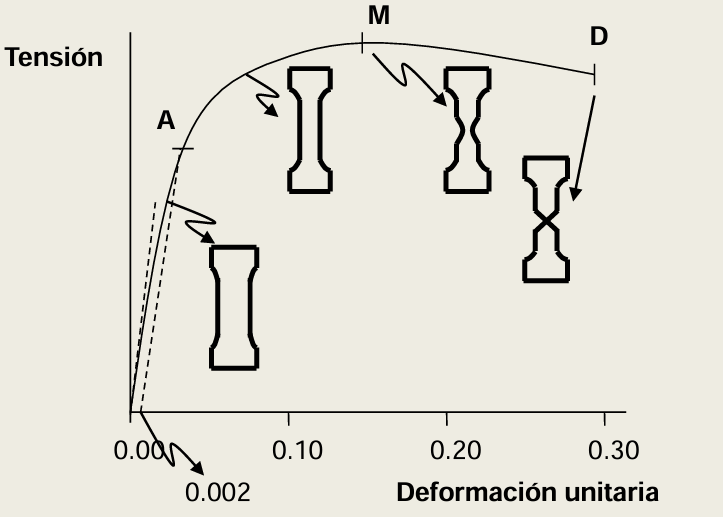
\includegraphics[width=0.7\textwidth]{punto_rotura.png}
    \caption{Resistencia máxima y punto de rotura \\ Fuente: Transparencias Asignatura}
    \label{fig:punto_rotura}
\end{figure}
\subsubsection{Ductilidad: Alargamiento y Estricción a la Rotura}
\dfn{Ductilidad:}{Grado de deformación plástica que puede soportar un material antes de su fractura.}
La ductilidad se determina cuantitativamente mediante el Alargamiento a la rotura (AR) y la Estricción a la rotura (ER) a partir de los datos obtenidos tras un ensayo de tracción con las siguientes expresiones:
\begin{enumerate}
    \item \textbf{Porcentaje de alargamiento a la rotura (\%AR):}
          \begin{equation}
              \%AR = \frac{l_f - l_0}{l_0} \times 100
              \label{eq:porcentaje_ar}
          \end{equation}
    \item \textbf{Porcentaje de estricción (\%ES):}
          \begin{equation}
              \%ES = \frac{A_0 - A_f}{A_0} \times 100
              \label{eq:porcentaje_es}
          \end{equation}
\end{enumerate}
donde $l_0$ y $A_0$ son la longitud calibrada y la sección inicial, y $l_f$ y $A_f$ son la longitud final entre puntos calibrados y la sección transversal mínima en el cuello de rotura.
\nt{A mayores valores de \%AR y \%ES, mayor es la ductilidad del material y su seguridad frente a roturas catastróficas.}
\begin{itemize}
    \item \textbf{Material frágil:} aquel que no puede tener apenas deformación plástica antes de romperse, se rompen de golpe, sin avisar. Por ejemplo el vidrio. Los materiales frágiles son aquellos que no han sufrido deformación plástica antes de romperse (se rompen justo en el límite elástico).
    \item \textbf{Material dúctil:} aquel que puede tener grandes deformaciones plásticas antes de romperse
\end{itemize}
\subsubsection{Resiliencia y Módulo de Resiliencia}
\dfn{Resiliencia:}{Es la capacidad de un material de absorber energía elástica cuando es deformado y devolverla íntegramente al retirar la carga exterior.}
\nt{Representa el área bajo el tramo elástico de la curva tensión-deformación hasta el límite de proporcionalidad.}

La energía de deformación elástica acumulada en el volumen de la probeta es el trabajo desarrollado por la fuerza:
\begin{equation}
    U = \frac{1}{2} P_{LP} \, \delta_{LP} \quad \xRightarrow{\text{Con la def. de }\sigma_{LP} \text{ y la ley de Hooke}} \frac{1}{2} \left(\frac{\sigma_{LP}^2}{E}\right) A_0 \, L_0
\end{equation}
El \textbf{Módulo de Resiliencia} ($U_r$) se define como la energía elástica absorbida por unidad de volumen de material:
\begin{equation}
    U_r = \frac{U}{A_0 \, L_0} = \frac{1}{2} \, \frac{\sigma_{LP}^2}{E}
    \label{eq:modulo_resiliencia}
\end{equation}
\textbf{Esta propiedad cuantifica la resistencia frente a choques a baja velocidad} y para maximizarla se requieren materiales con elevado límite elástico $\sigma_{LP}$ y bajo módulo elástico $E$.

\subsubsection{Tenacidad y Ensayos de Impacto (Charpy e Izod)}
\dfn{Tenacidad:}{Es la capacidad de un material de absorber energía mecánica elástica y plástica antes de que se produzca la fractura.}
Representa la energía máxima absorbida por unidad de volumen antes de originarse la ruptura total del material, se puede obtener de las siguientes formas:
\begin{itemize}
    \item Corresponde al área total bajo la curva completa tensión-deformación hasta el punto de rotura. Puede estimarse analíticamente de forma aproximada mediante la regla del trapecio:
          \begin{equation}
              \text{Tenacidad} \approx \frac{\sigma_A + \sigma_M}{2} \cdot \delta_D
              \label{eq:tenacidad_aprox}
          \end{equation}
          donde $\sigma_A$ es la tensión de fluencia, $\sigma_M$ la resistencia última y $\delta_D$ la deformación total a rotura.
    \item Evaluada mediante \textbf{ensayos normalizados de impacto en probetas entalladas (ensayos Charpy e Izod)}. Un martillo pendular de masa conocida se libera desde una altura inicial $h$, fractura la probeta entallada por flexión en un único golpe y asciende hasta una altura residual $h' < h$. La energía absorbida en el impacto es:
          \begin{equation}
              E_{\text{impacto}} = m g (h - h')
          \end{equation}
          \begin{itemize}
              \item \textit{Ensayo Charpy:} La probeta se apoya como viga simplemente apoyada en ambos extremos y el péndulo golpea en el centro por la cara opuesta a la entalla. Se utiliza típicamente en materiales dúctiles y aceros estructurales.
              \item \textit{Ensayo Izod:} La probeta se empotra verticalmente en voladizo y el péndulo golpea a una distancia fija en la cara donde se ubica la entalla. Muy empleado para plásticos y materiales más frágiles.
          \end{itemize}
\end{itemize}
\imp{La diferencia entre ambos ensayos es la forma de colocar la probeta. El ensayo de Izod se utiliza para determinar la tenacidad en materiales frágiles y el de Charpy para materiales dúctiles, ademas los resultados de los ensayos son cualitativos y se realizan con fines comparativos.}
\begin{figure}[H]
    \centering
    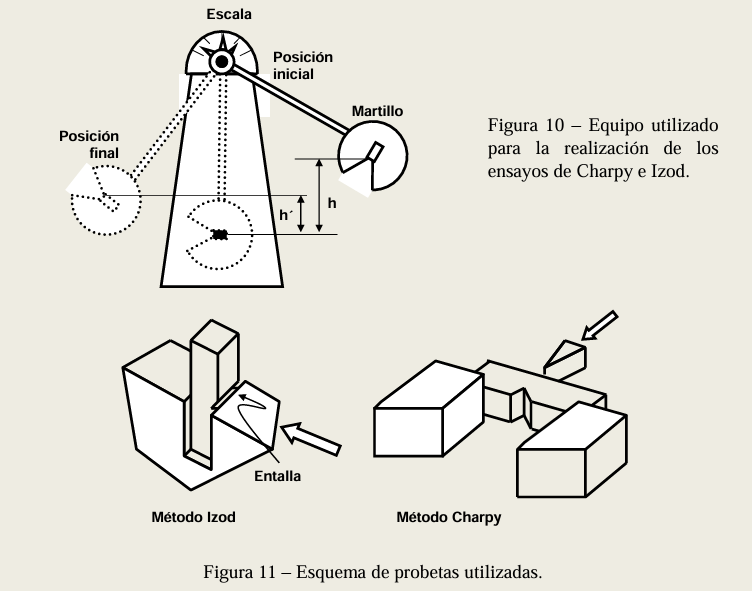
\includegraphics[width=0.6\textwidth]{ensayo_charpy_e_izod.png}
    \caption{Esquema del ensayo de \textbf{Charpy e Izod} \\ Fuente: Transparencias Asignatura}
    \label{fig:ensayo_charpy_e_izod}
\end{figure}
\paragraph{Transición Dúctil-Frágil y Efecto de la Temperatura:}
En metales con estructura cristalina cúbica centrada en el cuerpo (\textbf{BCC}, como los aceros al carbono ferríticos), la energía absorbida cae drásticamente al disminuir la temperatura, pasando de un comportamiento dúctil a alta absorción de energía a una rotura frágil y quebradiza por exfoliación a bajas temperaturas. Por el contrario, los metales con estructura cúbica centrada en las caras (\textbf{FCC}, como los aceros inoxidables austeníticos, aluminio, cobre y níquel) no presentan una transición brusca y retienen excelente tenacidad incluso a temperaturas criogénicas.

Asimismo, el contenido de carbono afecta de forma acusada: a medida que aumenta el porcentaje de carbono en los aceros recocidos, el material se vuelve más frágil, absorbe menos energía en el ensayo Charpy y el rango de transición hacia la fragilidad se desplaza a temperaturas más elevadas.
\imp{Es decir, en estos ensayos es importante la temperatura ya que puede haber una transición de ductil a fragil (cuando desciende la temperatura), ademas si cambiamos el contenido en carbono de los aceros recocidos se vuelven mas quebradizos y son capaces de absorber menos energía antes de su rotura.}
\begin{figure}[H]
    \centering
    \begin{subfigure}[c]{0.67\textwidth}
        \centering
        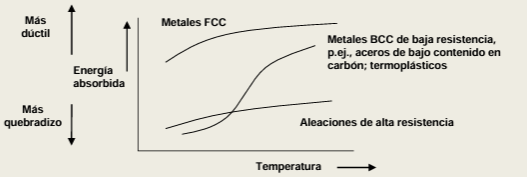
\includegraphics[height=4.2cm]{ductil_temperatura.png}
        \caption{Efecto de la temperatura en la tenacidad}
        \label{fig:ductil_temperatura}
    \end{subfigure}
    \hfill
    \begin{subfigure}[c]{0.3\textwidth}
        \centering
        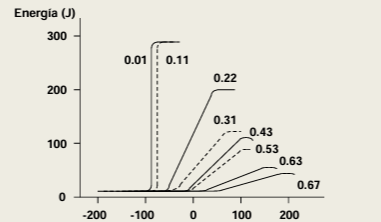
\includegraphics[height=4.2cm]{ductil_composicion.png}
        \caption{Efecto del porcentaje de carbono}
        \label{fig:ductil_composicion}
    \end{subfigure}
    \caption{Factores que influyen en la transición dúctil-frágil}
    \label{fig:ductil_transicion}
\end{figure}

\subsection{Tensiones y Deformaciones Reales}
En el cálculo convencional de ingeniería se utilizan el esfuerzo ingenieril $\sigma = P/A_0$ y la deformación ingenieril $\varepsilon = \delta/L_0$, es decir, se asume la sección inicial transversal a la aplicación de la carga para todos los calculos. Esto genera la falsa apariencia gráfica de que, superada la resistencia máxima, el material resiste menos esfuerzo. En la realidad física, el área transversal instantánea $A_i$ en la zona de estricción disminuye mucho más rápido que la carga aplicada, de modo que la tensión verdadera que soporta el material, \textbf{aumenta monótonamente hasta la rotura.}
\begin{figure}[H]
    \centering
    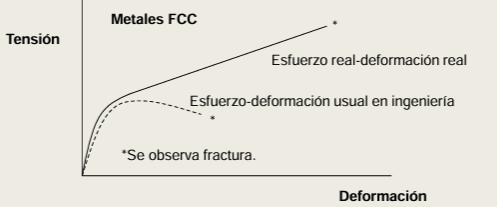
\includegraphics[width=0.7\textwidth]{deformacion_real.png}
    \caption{Tensión real vs Tensión ingenieril \\ Fuente: Transparencias Asignatura}
    \label{fig:deformacion_real}
\end{figure}
Se definen la \textbf{tensión real} ($\sigma_T$) y la \textbf{deformación real logarítmica} ($\varepsilon_T$) como:
\begin{equation}
    \sigma_T = \frac{P}{A_i}, \qquad \varepsilon_T = \int_{l_0}^{l_i} \frac{dl}{l} = \ln\left(\frac{l_i}{l_0}\right)
    \label{eq:tension_deformacion_reales}
\end{equation}
Asumiendo constancia de volumen durante la deformación plástica ($A_0 l_0 = A_i l_i$), se obtienen las relaciones de conversión válidas \textbf{hasta el comienzo de la estricción}:
\begin{equation}
    \sigma_T = \sigma \, (1 + \varepsilon), \qquad \varepsilon_T = \ln(1 + \varepsilon)
    \label{eq:conversion_real_nominal}
\end{equation}
\nt{Es decir que la tensión y deformación real estan relacionadas con las nominales(engenieriles) hasta que la probeta comienza a sufrir estricción.}
\paragraph{Ecuación constitutiva de Hollomon:}
En muchos metales y aleaciones, la región plástica comprendida entre el límite de fluencia y el comienzo de la estricción se ajusta fielmente a la ley potencial:
\begin{equation}
    \sigma_T = K \, \varepsilon_T^n
    \label{eq:hollomon}
\end{equation}
donde $K$ es el coeficiente de resistencia del material y $n$ es el \textbf{exponente de endurecimiento por deformación} ($n < 1$). A mayor valor de $n$, mayor es la capacidad del material para deformarse plásticamente de forma uniforme antes de que comience a localizarse la estricción (Tabla~\ref{tab:constantes_hollomon}).

\begin{table}[H]
    \centering
    \begin{tabular}{lcc}
        \toprule
        \textbf{Material}                     & \textbf{Exponente $n$} & \textbf{Constante $K$ ($\text{MPa}$)} \\
        \midrule
        Acero bajo en carbono (recocido)      & 0.26                   & 530                                   \\
        Acero aleado AISI 4340 (recocido)     & 0.15                   & 640                                   \\
        Acero inoxidable austenítico AISI 304 & 0.45                   & 1275                                  \\
        Aluminio recocido                     & 0.20                   & 180                                   \\
        Cobre recocido                        & 0.54                   & 315                                   \\
        Latón 70Cu-30Zn (recocido)            & 0.49                   & 895                                   \\
        Aleación de aluminio 2024-T4          & 0.16                   & 690                                   \\
        \bottomrule
    \end{tabular}
    \caption{Parámetros de endurecimiento por deformación ($n$ y $K$) para diversos materiales.}
    \label{tab:constantes_hollomon}
\end{table}

\subsection{Endurecimiento por Deformación Plástica (Acritud)}
Cuando un metal dúctil se somete a deformación plástica en frío (por encima de su límite elástico), la densidad de dislocaciones en su red cristalina se incrementa enormemente, multiplicándose y entorpeciendo su propio movimiento. \textbf{Es decir sufre una deformación plastica que produce un incremento de la resistencia elástica, tambien disminuye su ductilidad y aumenta su punto de fluencia.}

Si durante un ensayo de tracción se interrumpe la carga tras alcanzar una deformación plástica y se descarga el espécimen, el material desciende con una pendiente idéntica a la elástica ($E$). Al volver a aplicar carga, el material recorre el mismo camino elástico hasta alcanzar un \textbf{nuevo límite de fluencia significativamente más elevado} que el original.
\begin{figure}[H]
    \centering
    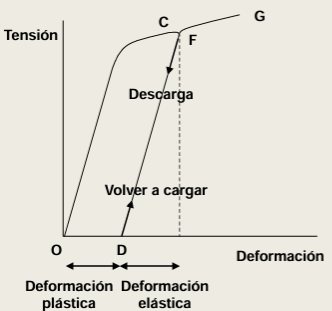
\includegraphics[width=0.5\textwidth]{endurecimiento_por_deformacion.png}
    \caption{Endurecimiento por deformación \\ Fuente: Transparencias Asignatura}
    \label{fig:endurecimiento_por_deformacion}
\end{figure}
\nt{En este grafico se observa como se le aplica una tensión inicial hasta recorriendo desde O hasta C, luego se descarga siguiendo la linea CD ya que al haber sufrido una deformación plastica no puede volver al estado original, siguiendo la trayectoria CD, al aplicar otra vez tensión seguira la trayectoria DF, siguiendo la ley de hooke hasta llegar a F y posteriormente si se sigue tensando habra un cambio brusco hasta G donde rompera.}
Este fenómeno confiere al material:
\begin{itemize}
    \item \textbf{Mayor rigidez y tensión elástica de servicio:} Se pueden aplicar cargas más altas sin que se genere nueva deformación plástica.
    \item \textbf{Aumento de la resistencia mecánica:} mejora unidireccional hacia donde se le aplico la carga, pero no mejora en el resto de las direcciónes del espacio.
    \item \textbf{Disminución de la ductilidad y de la tenacidad:} El material se torna más quebradizo.
    \item \textbf{Incremento del limite de proporcionalidad:} Aumenta la tensión necesaria para que el material comience a deformarse plásticamente.
    \item \textbf{Anisotropía:} El incremento de resistencia se produce preferentemente en la dirección en la que se aplicó la deformación uniaxial, pero no en las direcciones transversales.
    \item \textbf{Mayor susceptibilidad a la corrosión:} Las zonas con deformación plástica concentran tensiones residuales internas que aceleran la corrosión bajo tensión (aparece fluencia en las zonas no deformadas plásticamente).
\end{itemize}
El endurecimiento por deformación se puede revertir completamente restituyendo la ductilidad inicial mediante un \textbf{tratamiento térmico de recocido} a temperatura adecuada (tratamiento térmico suave a 100°C y posteriormente dejar enfriar lentamente).
\nt{Este tipo de tratamiento es común en procesos como el laminado de barras, estirado de tubos, ya que muchas veces se usa un material pretensado, es decir, se ha endurecido por acritud como se ha descrito previamente, un ejemplo sería en los pilares de hormigón pretensado, los cuáles son sometidos a esfuerzos de tracción para que se vuelvan más resistentes en dirección hacia donde sufrio la carga, aunque esto tiene un mayor coste economico.}
\section{Ensayo de Termofluencia (\textit{Creep})}

Muchos equipos de instalaciones químicas (\textbf{Reactores,turbinas}, calderas, intercambiadores de calor, columnas de destilación a presión y álabes de turbinas) operan simultáneamente bajo elevados esfuerzos mecánicos y altas temperaturas. A temperaturas elevadas las propiedades de los materiales experimentan cambios drásticos:
\begin{itemize}
    \item El módulo de elasticidad $E$ disminuye paulatinamente.
    \item El límite de proporcionalidad y la resistencia máxima a la tracción caen de forma notable a partir de cierta temperatura crítica.
    \item La ductilidad (\%AR y \%ES) se incrementa de forma acusada.
\end{itemize}

En estos equipos al sufrir una variación de temperatura importante, y tambien variación de presión (en especial en los reactores químicos de alta presión) las propiedades de los materiales pueden cambiar drásticamente, por lo que es importante conocer su comportamiento con este ensayo.

\subsection{Ensayo de tensión-deformación a distintas temperaturas}
\begin{figure}[H]
    \centering
    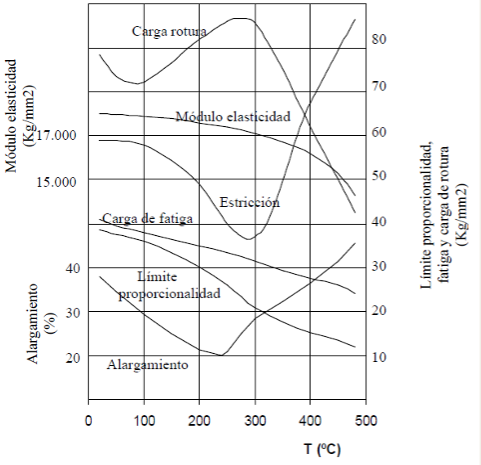
\includegraphics[width=0.5\textwidth]{termofluencia.png}
    \caption{Curva típica de termofluencia}
    \label{fig:termofluencia}
\end{figure}
En esta gráfica se puede observar la variación de las propiedades con la temperatura:
\begin{itemize}
    \item \textbf{Resistencia máxima a la tracción:} Crece hasta los 250\,°C.
    \item \textbf{Módulo de elasticidad:} Disminuye paulatinamente conforme aumenta la temperatura.
    \item \textbf{Contracción superficial (estricción):} Pasa por un mínimo a los 250\,°C y posteriormente crece de forma rápida.
    \item \textbf{Carga de fatiga:} Disminuye con la temperatura.
    \item \textbf{Límite de proporcionalidad:} Disminuye continuamente.
    \item \textbf{Alargamiento a la rotura:} Sigue un camino paralelo a la estricción ya que ambos definen la ductilidad (aumentan con la temperatura).
\end{itemize}

Los resultados de este ensayo arrojan la siguiente información:
\begin{itemize}
    \item Aquellas \textbf{propiedades que definen la ductilidad, como son la estricción y el alargamiento a la rotura, aumentan con la temperatura}
    \item las \textbf{propiedades relacionadas con la rigidez del material, como el límite de proporcionalidad y el módulo de elasticidad, disminuyen. La resistencia máxima a la tracción disminuye de forma apreciable tras una temperatura en específica}
\end{itemize}

\nt{En este gráfico se puede observar como la \textbf{resistencia a la tracción}} aumenta hasta los 250\,°C, mientras que el \textbf{módulo de elasticidad} disminuye de forma apreciable tras los 250\,°C, cabe mencionar que las \textbf{propiedades que definen la ductilidad, como son la estricción y el alargamiento a la rotura, aumentan con la temperatura}. Finalmente la \textbf{carga de fatiga} disminuye tras los 250\,°C.

Es importante considerar el tiempo como variable, ya que este ensayo es valido siempre y cuando  la carga actue durante un corto periódo de tiempo, si aumenta la duración (dias/semanas/meses) la carga necesaria para producir la rotura del material es cada vez mas pequeña.

\imp{para cargas que van a actuar durante largos períodos de tiempo y a temperaturas elevadas se necesitará una información más completa obtenida a partir de los ensayos termofluencia.}

\subsection{Ensayo de Termofluencia}
Bajo estas condiciones, la \textbf{variable tiempo} adquiere una importancia crítica. \textbf{Una pieza sometida a un esfuerzo constante inferior a su límite elástico puede sufrir una deformación plástica durante un cierto periodo de tiempo, esta deformación que depende del tiempo es conocida como termofluencia o fluencia lenta (\textit{creep})}.

\subsection{Curva Típica de Termofluencia y sus Etapas}
En un \textbf{ensayo} normalizado de \textbf{termofluencia}, una probeta se mantiene bajo \textbf{temperatura} rigurosamente controlada y \textbf{tensión} mecánica \textbf{constante}, registrando la \textbf{deformación en función del tiempo}. La curva característica presenta tres etapas bien diferenciadas:
\begin{enumerate}
    \item \textbf{Deformación elástica instantánea:} Es una deformación elástica instantánea que ocurre en el momento de aplicar la carga.
    \item \textbf{Etapa primaria o transitoria:} La probeta experimenta una deformación que aumenta progresivamente con el tiempo. el metal se endurece para soportar la carga aplicada por deformación, decreciendo la rapidez de la termofluencia con el tiempo a medida que el endurecimiento por deformación se hace más elevado.
    \item \textbf{Etapa secundaria o estacionaria:} La velocidad de deformación se mantiene prácticamente constante y mínima ($d\varepsilon/dt = \text{cte}$). En esta fase se establece un equilibrio dinámico entre el endurecimiento por deformación y los procesos térmicos de restauración y aniquilación de dislocaciones móviles promovidos por la difusión atómica. Tanto que el metal continúa alargandose a una velocidad constante, \textbf{La pendiente de esta región se denomina mínima rapidez de termofluencia}.
    \item \textbf{Etapa terciaria:} La velocidad de deformación se acelera de manera exponencial debido a la aparición de estricción macroscópica y la nucleación de microcavidades y grietas en los límites de grano, conduciendo rápidamente a la fractura del componente.
\end{enumerate}

la forma de la curva depende estrechamente de la carga y temperatura aplicada, Si existen esfuerzos y temperaturas elevadas, el tiempo necesario para la fractura del material disminuye de forma considerable.
\nt{Existen dos fenómenos importantes durante este proceso, un \textbf{endurecimiento del material provocado por la deformación plástica y un reblandecimiento causado al estar sometido a temperaturas elevadas.}}
\begin{figure}[H]
    \centering
    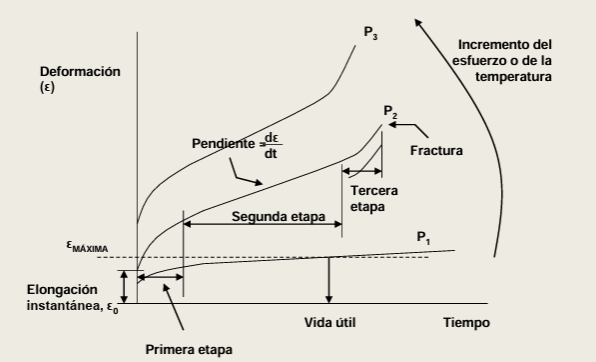
\includegraphics[width=0.7\textwidth]{ensayo_termofluencia.png}
    \caption{Curva típica de termofluencia}
    \label{fig:ensayo_termofluencia}
\end{figure}
Este ensayo se hace para materiales que soportaran altas temperaturas y cargas, como una turbina un reactor\dots
\imp{\textbf{La pendiente de la segunda etapa de la curva de termofluencia} es una medida que permite la comparación de diferentes materiales sometidos a las mismas condiciones del ensayo. El valor menor de la mínima rapidez de termofluencia una menor velocidad de deformación en esas condiciones.}
\nt{El esfuerzo que produce una \textbf{mínima rapidez de termofluencia de $10^{-5}\%/\text{h}$} también es otro parámetro que puede determinar la resistencia a la termofluencia e indicaría la evaluación de la carga máxima a aplicar al material a una determinada temperatura para que su velocidad de deformación fuese pequeña. \textbf{La elección de un material para trabajar a esfuerzo y temperaturas elevadas necesita de la realización de ensayos de termofluencia.} Este ensayo, junto con la \textbf{vida útil} del elemento, permite determinar fácilmente la \textbf{carga máxima} que puede ser aplicada sobre el material}
\section{Ensayo de Fatiga}

La \textbf{fatiga} es un mecanismo de degradación y \textbf{rotura} progresiva que se produce en piezas y componentes sometidos a tensiones dinámicas repetitivas, cíclicas o fluctuantes, por lo que el material falla con tensiones mucho mas pequeñas de las que podria soportar el material cuando se somete a cargas de tracción. \textbf{Es la primera causa de rotura de los materiales}

\textbf{Relevancia en ingeniería:} Representa la causa de más del $90\%$ de los fallos mecánicos en servicio en componentes metálicos. Lo más peligroso de la fatiga es que \textbf{la rotura sobreviene a tensiones notablemente inferiores a la resistencia estática de tracción e incluso por debajo del límite elástico, ocurriendo de forma súbita y sin deformación plástica previa apreciable}.

Las cargas aplicadas que producen fatiga pueden ser de distinta naturaleza: tracción, compresión, flexión o de naturaleza torsional. La resistencia que un material ofrece a la fatiga puede ser evaluada a partir de ensayos realizados en el laboratorio. Para ello la probeta se somete a esfuerzos alternativos de tracción y compresión de igual magnitud mediante el giro que provoca el equipo esquematizado, ademas las probetas son normalizadas. siguiendo el siguiente esquema
\nt{Suele ocurrir en equipos sometidos a presiones elevadas y tambien en ambientes corrosivos, otro ejemplo seria en un deposito donde se vacie y se llene continuamente.}
\subsection{Máquina de Ensayo y Curvas $S-N$ (Curvas de Wöhler)}
La resistencia a la fatiga se determina mediante ensayos dinámicos como el ensayo de flexión rotativa (máquina R.R.~Moore), en el que una probeta de sección calibrada gira a alta velocidad sometiéndose simultáneamente a tracción y compresión alternadas ($\sigma_{\text{med}} = 0$).

\begin{figure}
    \centering
    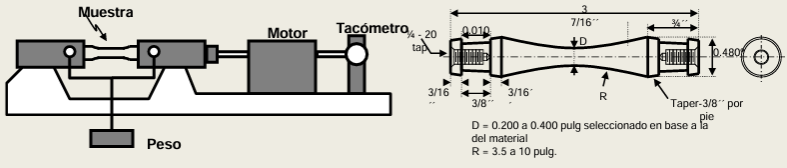
\includegraphics[width=0.7\textwidth]{ensayo_fatiga.png}
    \caption{Curva típica de fatiga}
    \label{fig:ensayo_fatiga}
\end{figure}

Los resultados se representan en un diagrama semilogarítmico de amplitud de tensión ($S$) frente al logaritmo del número de ciclos hasta la rotura ($N$):
\begin{itemize}
    \item \textbf{Materiales con límite de fatiga definido} (aceros al carbono y aleaciones de titanio): La curva $S-N$ se hace asintótica y totalmente horizontal a partir de un valor elevado de ciclos. Dicha asíntota define el \textbf{límite de fatiga} ($\sigma_e$ o $S_e$), que representa el nivel de tensión por debajo del cual el componente puede soportar un número infinito de ciclos sin romperse.
    \item \textbf{Materiales sin límite de fatiga definido} (aleaciones no férreas de aluminio, cobre, magnesio): La curva $S-N$ continúa descendiendo monótonamente. En este caso se define la \textbf{resistencia a la fatiga} para una vida prefijada de $N = 10^6$.
\end{itemize}

\begin{figure}
    \centering
    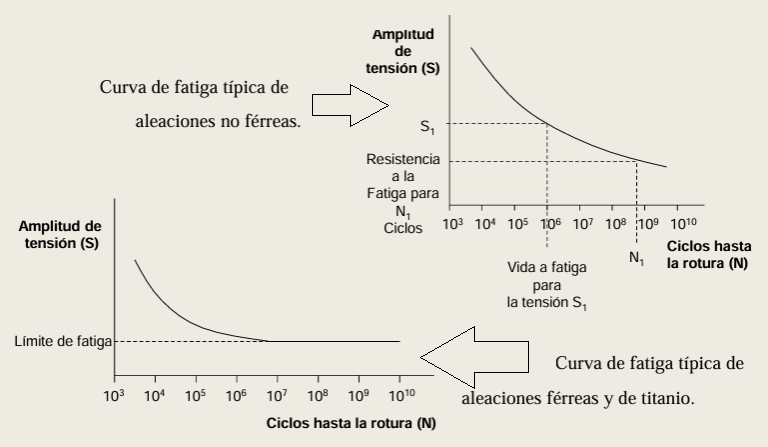
\includegraphics[width=0.7\textwidth]{curvas_fatiga.png}
    \caption{Curvas de fatiga para aleaciones ferricas y no ferricas. \\ Fuente: Callister, W. D. (2003). *Ciencia e Ingeniería de Materiales*. Grupo Editorial Iberoamericana.}
    \label{fig:curvas_fatiga}
\end{figure}
\imp{En resumen, los aceros al carbono y las aleaciones de titanio apresentam un límite de fatiga como la tensión para la cual el material puede someterse a infinitos ciclos. Otras aleaciones no férreas no presentan un límite de fatiga definido y para estos casos se define como la tensión de fatiga para la cual el material puede resistir hasta $10^6$ ciclos}
\subsection{Factores Críticos que Reducen la Vida a Fatiga}
La rotura por fatiga se inicia siempre en la superficie exterior y se propaga lentamente mediante microfisuras hasta la sección crítica restante. Los factores más determinantes son:
\begin{itemize}
    \item \textbf{Concentración de esfuerzos:} Entallas, ranuras, esquinas vivas, agujeros de paso o cambios bruscos de sección multiplican localmente las tensiones y actúan como iniciadores de grietas.
    \item \textbf{Rugosidad superficial:} Cuanto más pulida sea la superficie, mayor es la vida a fatiga; superficies rugosas o rayadas actúan como microentallas, cuanto mas pulido este el material el area superficial sera menor, y por tanto es menos susceptible a la corrosión y finalmente a la fatiga.
    \item \textbf{Ambiente de trabajo (fatiga-corrosión):} La presencia de medios agresivos mientras se aplican los esfuerzos ciclicos acelera la velocidad a la cual se propaga la fatiga.
    \item \textbf{Tratamientos superficiales protectores:} Procesos que modifican la superficie del material, por ejemplo aumentando la dureza superficial (como la nitruración o cementación) mejoran significativamente la resistencia a la fatiga \textbf{Debido a que la fatiga se inicia en la superficie del material}.
\end{itemize}

\nt{Dentro de los tratamientos superficiales, existe el tratamiento mecánico donde se modifica únicamente la superficie, tratamientos térmicos donde se modifica todo el material y tratamientos químicos como puede ser al pasar el material por gases después de una alta temperatura, consiguiendo así modificar las propiedades de las micras/mm de la superficie para evitar la fatiga.}
\section{Ensayo de Dureza (Propiedades Mecánicas Superficiales)}

\dfn{Dureza}{Es la propiedad mecánica superficial que mide la resistencia que opone un material a la deformación plástica localizada (una abolladura o arañazo).}


Históricamente se utilizó la escala cualitativa de \textbf{Mohs} (valores de 1 para el talco a 10 para el diamante, basada en la capacidad de rayado entre minerales). En ingeniería se utilizan \textbf{métodos cuantitativos normalizados} en condiciones controladas de carga y velocidad de aplicación de la carga, basados en el método de indentación (\textbf{mide la huella producida bien por profundidad o tamaño realizada por un penetrador sobre la superficie de un material}) y rayado:

\subsection{Métodos de Ensayo Cuantitativos}

\subsubsection{Dureza Rockwell (HR)}
Es el \textbf{método más utilizado para medir la dureza} debido a su simplicidad. Pueden utilizarse \textbf{diferentes escalas} con distintos penetradores y cargas, lo que permite que sirva para cualquier tipo de material, dúctil o frágil. Los penetradores son bolas esféricas de acero endurecido que tienen diámetros de $1/16$, $1/8$, $1/4$, $1/2$ pulgadas y un penetrador cónico de diamante que se utiliza para los materiales más duros. Se determina la dureza a partir de la diferencia de profundidad de la huella que resulta al aplicar primero una carga inicial pequeña y después una carga mayor. Los ensayos de dureza se realizan mediante equipos automatizados que determinan la diferencia de profundidad de forma automática tras la aplicación de las cargas. Existen \textbf{dos tipos de ensayos: Rockwell y Rockwell superficial}.
\begin{itemize}
    \item \textbf{Rockwell:} la carga inicial es de $10\text{ kg}$, mientras que las cargas mayores son $60$, $100$ y $150\text{ kg}$.
    \item \textbf{Rockwell superficial:} la carga inicial es de $3\text{ kg}$, mientras que las cargas mayores son $15$, $30$ y $45\text{ kg}$.
\end{itemize}
Estas escalas se identifican con un número que indica la carga y una letra que indica el penetrador utilizado. Cuando se especifican los ensayos de dureza se debe indicar el valor numérico de dureza que suele oscilar entre $100$ y $20$, recomendándose trabajar en este rango para que el ensayo sea correcto. Para ello se elige la carga y penetrador adecuado para cada material de forma que el valor de dureza esté comprendido entre esos valores. Así, una \textbf{dureza 80HRB significa dureza Rockwell (HR} o R en algunos casos) en \textbf{la escala B} (esfera de $1/16$ pulgadas y $100\text{ kg}$ de carga mayor) y \textbf{valor numérico de dureza de 80}.

\subsubsection{Dureza Brinell (HB)}
Utiliza un penetrador esférico de acero endurecido o carburo de tungsteno (típicamente de diámetro $D = 10\text{ mm}$ o $5\text{ mm}$) sobre el que se aplica una carga estática $P$ (entre $500$ y $3000\text{ kgf}$) durante un tiempo normalizado (entre $10$ y $30\text{ segundos}$).

\textbf{El número de dureza Brinell (HB)} se calcula dividiendo la carga aplicada por la superficie del casquete semiesférico de la huella de diámetro $d$:
\begin{equation}
    HB = \frac{2P}{\pi D \left(D - \sqrt{D^2 - d^2}\right)}
    \label{eq:dureza_brinell}
\end{equation}
\nt{La notación «Dureza Brinell» de $\text{HB}(5/1000/15)$ especifica que se empleó una esfera de $5\text{ mm}$, carga de $1000\text{ kgf}$ y tiempo de aplicación de $15\text{ s}$.}

\subsubsection{Microdureza Vickers (HV) y Knoop (HK)}
Emplean cargas muy reducidas (desde $1\text{ g}$ hasta $1000\text{ g}$) y penetradores de diamante piramidales; requiere una minuciosa preparación de la muestra mediante pulido:
\begin{itemize}
    \item \textbf{Vickers (HV):} Pirámide de base cuadrada con ángulo entre caras de $136^\circ$. La dureza es función de la media de las diagonales $d_1$ y $d_2$ de la huella observada al microscopio.
    \item \textbf{Knoop (HK):} Pirámide de base rómbica alargada; permite evaluar gradientes de dureza y capas superficiales extremadamente finas o materiales muy frágiles como los cerámicos.
\end{itemize}
\imp{Tanto Vickers como Knoop se utilizan para materiales frágiles como los cerámicos.}
\subsection{Conversión de la dureza}
Ya que la dureza no está normalizada, \textbf{no se ha establecido un método general para su conversión}. \textbf{Para aceros, la resistencia a la tracción y la dureza Brinell} están asociadas, por lo que se puede establecer una correlación empírica directa; se cumple con excelente aproximación:
\begin{equation}
    \sigma_M \, [\text{MPa}] \approx 3.45 \times HB \qquad \left(\sigma_M \, [\text{psi}] \approx 500 \times HB\right)
    \label{eq:relacion_dureza_resistencia}
\end{equation}

\section{Propiedades Tecnológicas de los Materiales}
\dfn{Propiedades Tecnológicas}{Son aquellas propiedades que están relacionadas con la capacidad que tienen los materiales para transformarse en cuerpos huecos y con la facilidad que estos tienen para ser mecanizados y modificar su forma.}

Para determinar sus propiedades se realizan los siguientes ensayos:
\begin{enumerate}
    \item \textbf{Soldabilidad:} Capacidad del material de resistir las alteraciones de su textura y las tensiones térmicas motivadas por el soldeo sin deterioro. Los ensayos consisten en unir piezas en condiciones similares a las reales y posteriormente \textbf{se examinan las uniones soldadas mediante ensayos de flexión para comprobar si la soldadura muestra la misma resistencia.} En el caso real se suelen tomar eficacias de soldadura donde la resistencia es ese coeficiente de corrección que multiplica la tensión de trabajo del material que se había determinado previamente a la soldadura.
    \item \textbf{Ensayo de flexión (doblado):} Se realiza para reconocer la flexibilidad de un material; se realiza en un ángulo comprendido entre $90^\circ$ y $180^\circ$. El material debe doblarse sin agrietarse.
    \item \textbf{Ensayo de torsión:} Determina la tenacidad y resistencia a cizalladura midiendo el número de vueltas completas que resiste una pieza cilíndrica antes de fracturarse. \textbf{El número de torsiones que resiste al girar una pieza determina su tenacidad (la pieza gira mientras está sujeta por un extremo).}
    \item \textbf{Embutición (Ensayo Erichsen):} Determina la \textbf{capacidad} de un material para \textbf{ser transformado en un cuerpo hueco} (fondos de reactores, depósitos o envolventes). Un pistón de cabeza semiesférica penetra contra la chapa sujeta perimetralmente; la profundidad de penetración hasta la primera grieta mide el índice de embutibilidad.
    \item \textbf{Ensayo de abocardado / ensanchamiento de tubos:} En el interior del tubo que se va a ensanchar se introduce mediante golpes a presión un cono engrasado; se observa posteriormente la aparición de fisuras en las paredes y la resistencia al ensanchamiento que ha manifestado el tubo.
    \item \textbf{Ensayo de estanqueidad de tubos:} Se someten los tubos a presión hidráulica de ensayo (típicamente $1.25$ a $1.5$ veces la presión máxima de servicio, en un fluido líquido) para verificar la total hermeticidad y ausencia de defectos en juntas soldadas (se martillea el tubo mientras está sometido a la presión para intentar provocar la aparición de fisuras y comprobar su estanqueidad).
\end{enumerate}

\section{Ensayos No Destructivos (END)}

\dfn{Ensayos No Destructivos}{Los Ensayos No Destructivos tienen por objeto \textbf{inspeccionar y caracterizar defectos e imperfecciones de piezas terminadas o que estén en servicio}.}

Las principales técnicas empleadas en el mantenimiento preventivo y control de calidad de plantas químicas comprenden:
\begin{itemize}
    \item \textbf{Inspección visual (VT):} Técnica básica directa u óptica mediante boroscopios para evaluar defectos superficiales macroscópicos, alineaciones y cordones de soldadura.
    \item \textbf{Líquidos penetrantes (PT):} Aplicación de tintas coloreadas o fluorescentes de baja tensión superficial para revelar fisuras y discontinuidades abiertas a la superficie en cualquier material no poroso.
    \item \textbf{Partículas magnéticas (MT):} Exclusivo para materiales ferromagnéticos; la fuga de campo magnético provocada por un defecto superficial o subsuperficial atrae finas partículas de hierro polarizadas haciéndolo visible.
    \item \textbf{Ultrasonidos (UT):} Emisión de ondas acústicas de alta frecuencia que se reflejan en las interfases y discontinuidades internas, permitiendo detectar grietas y medir espesores remanentes de pared por corrosión.
    \item \textbf{Radiografía y Gammagrafía (RT):} Radiaciones ionizantes (rayos X o isótopos gamma como $^{192}\text{Ir}$ o $^{60}\text{Co}$) que impresionan detectores, obteniendo una imagen volumétrica interna de soldaduras y piezas fundidas.
    \item \textbf{Corrientes inducidas (ET):} Detección de fallos y variaciones de conductividad en materiales conductores mediante corrientes de Foucault.
    \item \textbf{Emisiones acústicas (AE):} Detección pasiva en tiempo real del sonido emitido por la propagación de microfisuras durante pruebas de carga o presurización.
\end{itemize}

\nt{Se basan en la valoración de las distintas propiedades del material cuando existen perturbaciones estructurales que se comparan con las que tendrían si no hubiese esas perturbaciones.}
\section{Tensión de Trabajo y Factor de Seguridad}

Los ensayos anteriores hasta ahora se han realizado en \textbf{condiciones normalizadas y controladas} de laboratorio con probetas pulidas bajo condiciones ideales y uniaxiales. Sin embargo, en la realidad distan de las \textbf{condiciones de servicio} y los componentes operan bajo estados de tensión poliaxiales complejos, cargas fluctuantes, variaciones térmicas, corrosión y tolerancias de fabricación.

Para ello se define en el material una \textbf{tensión de seguridad o tensión de trabajo $\sigma_T$}.

Para diferentes situaciones esta \textbf{tensión de trabajo se evalúa a partir de la resistencia máxima a la tracción $\sigma_M$ o la tensión en el punto de fluencia $\sigma_A$ divididas por un coeficiente de seguridad $n$}:
\begin{equation}
    \sigma_T = \frac{\sigma_{\text{límite}}}{n}
    \label{eq:tension_trabajo}
\end{equation}
donde $\sigma_{\text{límite}}$ es la tensión de fluencia ($\sigma_A$) o la resistencia última a la tracción ($\sigma_M$), y $n$ es el \textbf{factor de seguridad} ($n > 1$).

\subsection{Criterios de Elección del Factor de Seguridad ($n$)}
El factor $n$ se selecciona en base a códigos de diseño (ASME, AISC, UNE), fluctuando habitualmente entre \textbf{$1.2$} y \textbf{$4.0$} (con un valor promedio típico de \textbf{$2.0$} para solicitaciones estáticas convencionales).

el factor de seguridad dependera del equipo que se vaya a usar
\begin{itemize}
    \item Un valor de $n$ excesivamente bajo compromete la seguridad y puede provocar fallos catastróficos.
    \item \textbf{Un valor excesivamente alto conduce a un diseño sobredimensionado}, multiplicando el peso propio de la instalación y su coste de fabricación.
\end{itemize}

\begin{table}[H]
    \centering
    \begin{tabular}{lcc}
        \toprule
        \textbf{Naturaleza de la Carga} & \textbf{Materiales Dúctiles}      & \textbf{Materiales Quebradizos / Frágiles} \\
        \midrule
        Carga estática                  & $\sigma_T = \dfrac{\sigma_A}{2}$  & $\sigma_T = \dfrac{\sigma_M}{6}$           \\[8pt]
        Carga repetitiva                & $\sigma_T = \dfrac{\sigma_M}{8}$  & $\sigma_T = \dfrac{\sigma_M}{10}$          \\[8pt]
        Carga de choque o impacto       & $\sigma_T = \dfrac{\sigma_M}{12}$ & $\sigma_T = \dfrac{\sigma_M}{15}$          \\
        \bottomrule
    \end{tabular}
    \caption{Criterios habituales de cálculo de la tensión de trabajo para esfuerzos normales directos.}
    \label{tab:criterios_esfuerzo_diseno}
\end{table}

\subsection{Criterios de Reglamentos Específicos para Cargas Estáticas}
\begin{itemize}
    \item \textbf{Acero estructural (AISC - \textit{American Institute of Steel Construction}):}
          \begin{equation}
              \sigma_T = \text{min}\left\{\frac{\sigma_A}{1.67} \approx 0.60 \, \sigma_A, \quad \frac{\sigma_M}{2.0} = 0.50 \, \sigma_M\right\}
              \label{eq:criterio_aisc}
          \end{equation}
    \item \textbf{Aleaciones de aluminio (Aluminum Association):}
          \begin{equation}
              \sigma_T = \text{min}\left\{\frac{\sigma_A}{1.65} \approx 0.61 \, \sigma_A, \quad \frac{\sigma_M}{1.95} \approx 0.51 \, \sigma_M\right\}
              \label{eq:criterio_aa}
          \end{equation}
\end{itemize}
